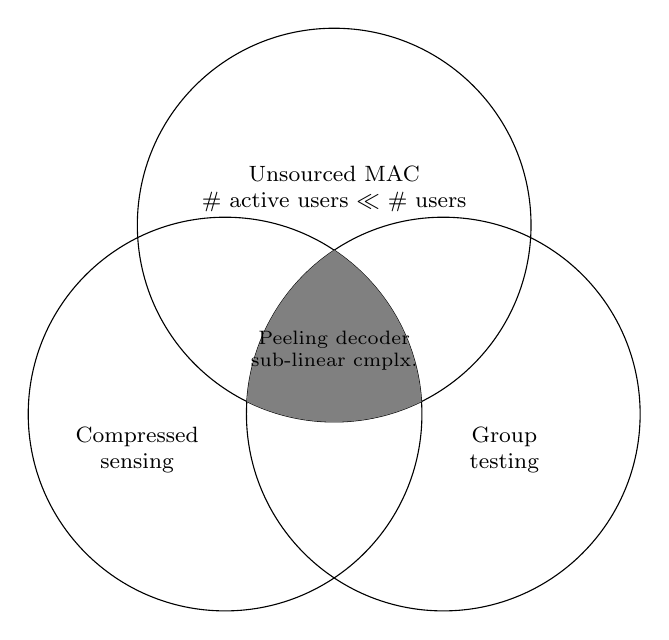
\begin{tikzpicture}
\def\fsize{\footnotesize}
\def \r{2.5cm}
\def\dist{1.6cm}

	\def\firstcircle{(90:\dist) circle (\r)}
  	\def\secondcircle{(210:\dist) circle (\r)}
	 \def\thirdcircle{(330:\dist) circle (\r)}
  
     \draw \firstcircle node[text=black,anchor=south] {
	\fsize{\begin{tabular}{c}
	 Unsourced MAC\\
	$\#$ active users $\ll$ $\#$ users\\
    \end{tabular}}
     };
     
    \draw \secondcircle node[text=black,anchor=north east] { %\fsize{Compressed sesning}};
    \fsize{\begin{tabular}{c}
    Compressed \\
    sensing\\
    \end{tabular}}
    };
    \draw \thirdcircle node[text=black,anchor=north west] {
        \fsize{\begin{tabular}{c}
	Group\\ testing\\ 
  \end{tabular}}
};
  
    
   \begin{scope}
    \clip \firstcircle;
    \clip \secondcircle;
    \fill[gray] \thirdcircle;
      \end{scope}
      
      
	\node (center) at (0,0) {
	         \scriptsize{\begin{tabular}{c}
	 Peeling decoder\\
	 sub-linear cmplx.\\	
	\end{tabular}}
	};
	
	
	
	
  \end{tikzpicture}